\chapter{Ergebnisse}

Zum Generieren der Ergebnisse wurde Grid-Search auf beiden Datensätzen für beide Ansätze, Klassifikation und
 Regressions-Ensemble, angewendet. Da dabei alle möglichen Kombinationen der Hyperparameter getestet werden,
 kann man einerseits verhindern, in lokale Optima zu laufen, andererseits kostet dieses Verfahren eine lange
 Zeit. Damit ist sowohl die Generierung, als auch die Analyse gemeint, da die Anzahl an Ergebnissen durch das
 Produkt der jeweils möglichen Einstellungen der Hyperparameter gegeben ist. Existieren beispielsweise fünf
 Hyperparameter mit jeweils fünf Einstellungen, so ist die Anzahl an Durchläufen gleich $5^5=3125$.
 Eine Auflistung, wie viele Kombinationen getestet wurden, kann in Tabelle \ref{tab:res-kombs} eingesehen werden.

 \begin{table}[h]
    \centering
    \begin{tabular}{l|ll|ll}
    & \multicolumn{2}{l|}{Klassifikation} & \multicolumn{2}{l}{Regression-Ensemble} \\
    \hline
    Basemodel & \# HP & \# Kombi. & \# HP & \# Kombi. \\
    \hline
    LR        &                           &                                & \multicolumn{1}{c}{0}     & \multicolumn{1}{c}{300}       \\
    Ridge     &                           \multicolumn{2}{c|}{-}           & \multicolumn{1}{c}{1}     & \multicolumn{1}{c}{1800}      \\
    Lasso     &                           &                                & \multicolumn{1}{c}{1}     & \multicolumn{1}{c}{1800}      \\
    kNN       & \multicolumn{1}{c}{2}     & \multicolumn{1}{c|}{40}        & \multicolumn{1}{c}{2}     & \multicolumn{1}{c}{2400}      \\
    MLP       & \multicolumn{1}{c}{3}     & \multicolumn{1}{c|}{900}       & \multicolumn{1}{c}{3}     & \multicolumn{1}{c}{54000}
    \end{tabular}
    \caption{Anzahl (als \# abgekürzt) von Hyperparametern (HP) einzelner Modelle und ihrer insgesamter Anzahl an
        Kombinationen inklusive der Wrapper-Klasse. Klassifikation besitzt nur einen Hyperparameter, während
        Regression-Ensemble vier besitzt.}
    \label{tab:res-kombs}
\end{table}

Da eine detaillierte Analyse aller Kombinationen den Rahmen dieser Arbeit sprengen würde, werden für den
 Ad-Hoc Datensatz sowie für den Ansatz der Klassifikation bei dem LeakDB Datensatz nur die besten Konfigurationen
 präsentiert. Da der Regressions-Ensemble-Ansatz auf dem realistischeren Datensatz die wichtigsten Werte zeigt,
 wird dieser detaillierter betrachtet. Hier wird zuletzt auch die Detektionszeit und das Feature Extraction
 analysiert. Die vollständigen Werte jedes einzelnen Experimentes sind auf der GitHub-Seite als csv-Dateien
 bereitgestellt [TODO Quelle]. Dort ist ebenfalls ein Notebook namens \texttt{analyse.ipynb} hinterlegt, in welchem
 die komplette Analyse der Ergebnisse dokumentiert ist.

\section{Optimale Konfiguration}

Im Zuge des Ad-Hoc Datensatzes wurden 300 Zeitfolgen mit jeweiliger Zeitspanne von fünf Tagen getestet. Um die
 Accuracy als valide, erste Einschätzung der Güte nutzen zu können, ist der Datensatz genau zur Hälfte in
 leckfreie und leckbehaftete Szenarien aufgeteilt. Abbildung \ref{fig:res-best-adhoc} zeigt die Metriken der, nach
 Accuracy, besten Konfigurationen der jeweiligen Ansätze und Basemodels. Anhang \ref{appendix-best-conf} listet
 die jeweiligen Werte auf. Wichtig zu bemerken ist, dass k-Nearest Neighbors in beiden Ansätzen und allen Metriken
 den höchsten Wert von 100\% abliefert. Währenddessen sind bei der Linearen Regression und vor allem bei der
 L2-Regulierung starke Einbrüche in der Sensitivität für Lecks zu sehen.

Um auch bei LeakDB die Accuracy nutzen zu können, wurden aus den 1000 Szenarien 500 ausgewählt, sodass diese
 mit 250 leckfreien zu 250 leckbehafteten Szenarien balanziert war. Zusätzlich zu der doppelten, zeitlichen
 Auflösung, ist jede Zeitfolge hier zehn Tage lang. Abbildung \ref{fig:res-best-leakdb} zeigt wieder die besten
 Werte auf, dessen Konfigurationen in Anhang \ref{appendix-best-conf} wieder gezeigt werden. Hier ist zu bemerken,
 dass kNN aus dem Ansatz des Regressions-Ensembles stark eingebrochen ist, während die anderen Werte weitgehend
 stabil bleiben.

\begin{figure}[h]
    \centering
    \begin{subfigure}{\textwidth}
        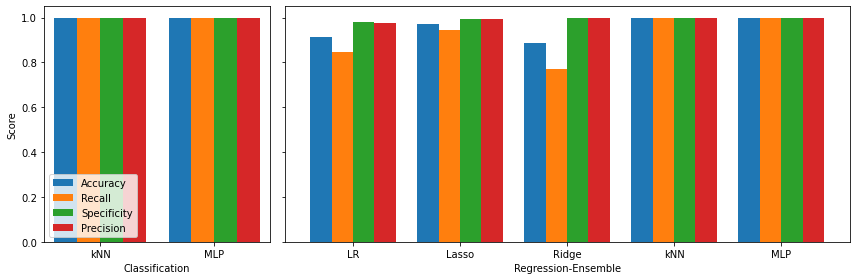
\includegraphics[width=1.0\textwidth]{res/res-best-adhoc}
        \caption{Ad-Hoc Datensatz\vspace{1em}}
        \label{fig:res-best-adhoc}
    \end{subfigure}
    \begin{subfigure}{\textwidth}
        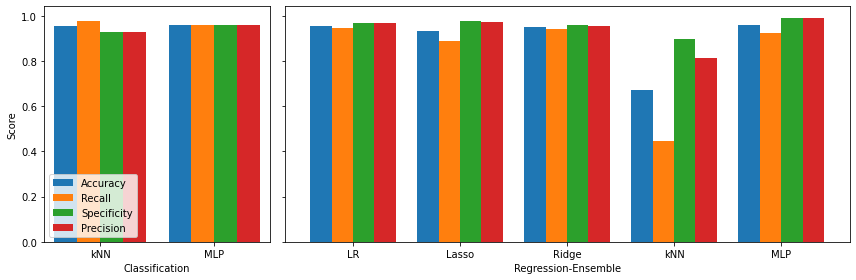
\includegraphics[width=1.0\textwidth]{res/res-best-leakdb}
        \caption{LeakDB}
        \label{fig:res-best-leakdb}
    \end{subfigure}
    \caption{Die Werte der besten Konfigurationen einzelner Modelle, nach der Akkuratheit.}
\end{figure}

\section{LeakDB Datensatz}

Um diese massiven Datenmengen analysieren zu können, wurde zuerst für jeden Hyperparameter ein Einfluss-Wert
 erzeugt. Dieser gibt Aufschluss darüber, wie viel Einfluss die Veränderung dieses Wertes auf das Ergebnis
 einer Metrik hat und wird wie folgt berechnet:

\begin{verbatim}
    def influence(results, feature, metric='accuracy'):
        grouped = results.groupby(feature).mean().loc[:, metric]
        return grouped.max() - grouped.min()
\end{verbatim}

Hierbei sind \texttt{results} die Ergebnisse aus der csv-Datei, \texttt{feature} das zu untersuchende Feature
 und \texttt{metric} die jeweilige Metrik. Die \texttt{groupby}-Funktion gruppiert also zuerst die Ergebnisse
 nach dem Hyperparameter, dessen Einfluss berechnet werden soll. Für jede seiner möglichen Einstellungen wird
 dann der mittlere Metrikwert berechnet, was dazu führt, dass die Differenz des maximalen zu dem minimalen
 Mittelwert den Gesamteinfluss widerspiegelt. Ein Hyperparameter mit einem Einfluss von 0.6 hat also das
 Potential, das Ergebnis um 0.6, also 60\%-Punkte, zu verändern, während ein Hyperparameter mit einem Einfluss
 von 0.01 nur wenig am Endergebnis verändern kann. Anhang \ref{appendix-ranking} gibt den Einfluss jedes
 möglichen Hyperparameters pro Basemodel an. Hier ist gut zu sehen, dass der Wrapper-spezifische Hyperparameter
 \texttt{th\_majority}, also die Anzahl, wie viele Knoten Alarm schlagen müssen, bevor ein Zeitpunkt als
 leckbehaftet gilt, tendenziell den größten Effekt auf das Endergebnis hat, während die Größe des Median-Filters
 nur einen sehr kleinen Effekt hat. Für kNN und MLP ist \texttt{th\_majority} jedoch nur an zweiter Stelle, da
 ihre modellspezifischen Hyperparameter \texttt{weights} und \texttt{activation} größeren Einfluss haben.

Die folgenden Analysen der Hyperparameter wurden generiert, indem die Hyperparameter mit höherem Einfluss auf
 ihre lokale Optima gesetzt wurden und die Werte der Hyperparameter geringerem Einflusses gemittelt wurden.
 So lassen sich Tendenzen in der Veränderung eines Hyperparameters isolierter betrachten. Alle Grafiken dieser
 Analyse sind im Anhang gezeigt, welche keine Korrelation ergibt.

Schaut man sich zuerst den verhältnismäßig einflussreichsten Hyperparameter \texttt{th\_majority} an, so fällt auf,
 dass der Verlauf bei allen Basemodels ungefähr gleich ist. Abbildung \ref{fig:res-th-majority} zeigt dies am
 Beispiel des MLPs. Während die Spezifität annähernd konstant bleibt, sinken die Werte der Sensitivität und
 Akkuratheit. Am interessantesten ist die Präzision, also der Anteil echter Lecks an den prognostizierten Lecks,
 welcher erst Nahe eins bleibt, dann aber plötzlich stark abfällt. Ein weiterer, einflussreicher
 Wrapper-Hyperparameter ist \texttt{th\_mode}, welche die Abhängigkeit der Thresholds von der Tageszeit einstellt.
 Auch hier sind die Verläufe ähnlich unter den Basemodels und liefert ein klares Bild: Die Thresholds von der
 Tageszeit abhängig zu machen verbessert die Akkuratheit und die Sensitivität, während die anderen Metriken sich
 nur leicht verschlechtern, wie am Beispiel der Linearen Regression in Abbildung \ref{fig:res-th-mode} zu sehen
 ist. Weniger Einfluss geht von \texttt{th\_multiplier} aus, welcher die berechneten Thresholds künstlich erhöhen
 kann. Abbildung \ref{fig:res-th-multiplier} zeigt die Interaktion mit \texttt{th\_majority} in einer Heatmap.

\begin{figure}
    \centering
    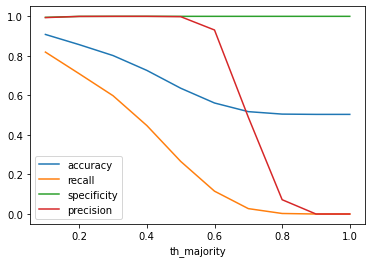
\includegraphics[width=0.7\textwidth]{res/res-th-majority}
    \caption{Durchschnittlicher Verlauf der Metriken für den Hyperparameter \texttt{th\_majority}.}
    \label{fig:res-th-majority}
\end{figure}

\begin{figure}
    \centering
    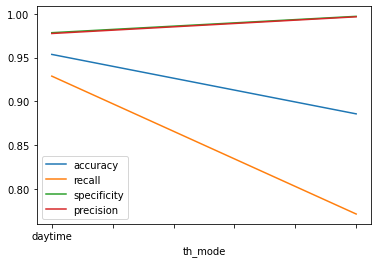
\includegraphics[width=0.7\textwidth]{res/res-th-mode}
    \caption{Durchschnittliche Werte der Metriken für \texttt{daytime} (links) und
        \texttt{simple} (rechts) des Hyperparameters \texttt{th\_mode}.}
    \label{fig:res-th-mode}
\end{figure}

\begin{figure}
    \centering
    \fbox{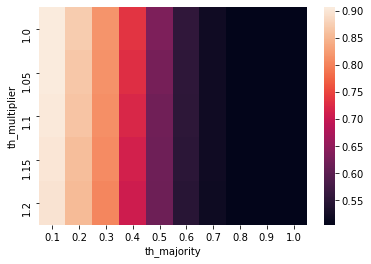
\includegraphics[width=0.7\textwidth]{res/res-th-multiplier}}
    \caption{2-dimensionaler Verlauf der Accuracy in Abhängigkeit der Hyperparameter \texttt{th\_multiplier} und
        \texttt{th\_majority} für die Ridge Regression.}
    \label{fig:res-th-multiplier}
\end{figure}

Für k-Nearest Neighbors ist der einflussreichste Hyperparameter \texttt{weights}, mit welchem angegeben werden
 kann, ob die Datenpunkte in der Nachbarschaft alle gleich gewichtet werden, oder nach ihrem Abstand. Der Effekt
 von distanzbasierter Gewichtung im Vergleich zur uniformen Gewichtung wird in Abbildung
 \ref{fig:res-knn-weights} gezeigt. Hier sieht man, dass die Spezifität abnimmt, während die Sensitivität
 erhöht wird. Bei der distanzbasierten Gewichtung werden also mehr Punkte als Leck klassifiziert.

\begin{figure}
    \centering
    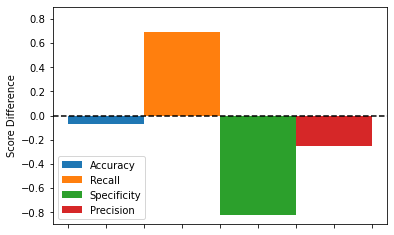
\includegraphics[width=0.7\textwidth]{res/res-knn-weights}
    \caption{Relative Veränderung der Metriken beim Umschalten auf distanzbasierten Gewichten für kNN.
        Sensitivität verbessert sich stark, während die Spezifität sich verschlechtert hat.}
    \label{fig:res-knn-weights}
\end{figure}

Betrachtet man das MLP, so ist die richtige Wahl der Aktivierungsfunktion am entscheidendsten. Abbildung
 \ref{fig:res-mlp-activation} zeigt, dass die Wahl der logistischen Funktion oder der Hyperbeltangens im
 Mittelwert zu einer Präzision und Sensitivität nahe null führt. Ein weiterer, nicht so einflussreicher
 Hyperparameter von MLP ist die Gestaltung der verborgenen Schichten. Auch, wenn es schwierig ist, eine Ordnung
 auf der Struktur zu finden, kann man in Abbildung \ref{fig:res-mlp-layers}, welche die Schichten zuerst nach
 ihrer Anzahl und dann ihrer Summe an Perzeptronen sortiert, einen kleinen Abwärtstrend in der Sensitivität
 sehen, je größer das künstliche, neuronale Netz ist.

\begin{figure}
    \centering
    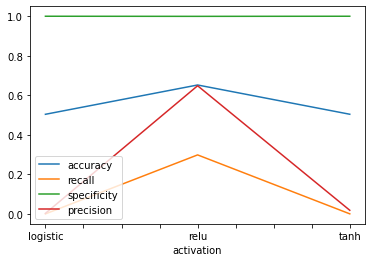
\includegraphics[width=0.7\textwidth]{res/res-mlp-activation}
    \caption{Durchschnittlicher Metrikwerte für die drei Aktivierungsfunktionen des MLPs.}
    \label{fig:res-mlp-activation}
\end{figure}

\begin{figure}
    \centering
    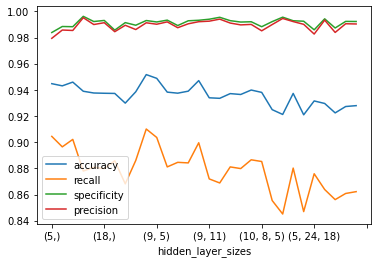
\includegraphics[width=0.7\textwidth]{res/res-mlp-layers}
    \caption{Durchschnittliche Metrikwerte abhängig von der Form der verborgenen Schichten.
        Dabei sind links tendenziell kleinere Netzwerke, während sie nach rechts wachsen.}
    \label{fig:res-mlp-layers}
\end{figure}


Für die meisten Hyperparameter ist das Optimum für die bisher betrachteten Metriken ebenso das der
 Detektionszeit. Ein davon abweichender Fall, welcher in Abbildung \ref{fig:res-fe-th-mode} gezeigt wird, ist der
 \texttt{th\_mode}, welcher im Gegensatz zu den anderen Metriken leicht die simple Einstellung bevorzugt.

\begin{figure}
    \centering
    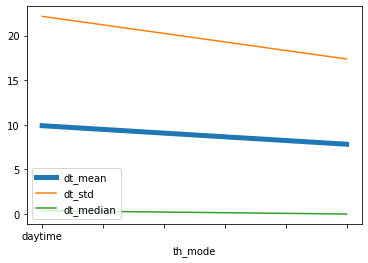
\includegraphics[width=0.7\textwidth]{res/res-fe-th-mode}
    \caption{Informationen über die Detektionszeit (dt) für \texttt{daytime} (links) und
        \texttt{simple} (rechts) des Hyperparameters \texttt{th\_mode} anhand Ridge.
        Dabei sind hier kleinere Werte besser, was \texttt{simple} etwas besser macht.}
    \label{fig:res-fe-th-mode}
\end{figure}

\section{Einfluss von Feature Extraction}

Um die Effekte der zwei Techniken der Feature Extraction zu analysieren wurde das Basemodel Ridge Regression
 für den Ansatz des Regression-Ensembles genutzt. Für die Past Days Transformation wurden Werte zwischen Eins,
 also keinem Rückblick, und Fünf, also ein Rückblick um bis zu vier Tage in die Vergangenheit, gewählt. Für
 die Mean Transformation wurde ebenso eine Fenstergröße von Eins, also keiner Veränderung, bis zu Fünf, also
 einer Mittelwertberechnung über fünf Werte, vorgegeben. Die Ergebnisse lassen sich als Heatmap in
 Abbildung \ref{fig:res-fe-metrics} einsehen. Interessant ist hier zu sehen, dass obwohl der Rückblick in die Vergangenheit generell
 bessere Werte liefert, so weiter dieser ist, ist für Accuracy und Sensitivity kein Rückblick am besten. Zudem
 kann die Mittelung der Werte nur bessere Werte hervorbringen, falls die Past Days Transform aktiv ist.

Betrachtet man sich jedoch die Detektionszeit in Abbildung \ref{fig:res-fe-dt}, so hat die Mittelung für die
 durchschnittliche Detektionszeit auch ohne Past Days Transform einen guten Effekt.

 \begin{figure}
    \centering
    \begin{adjustwidth}{-1cm}{}
        \begin{subfigure}{\textwidth}
            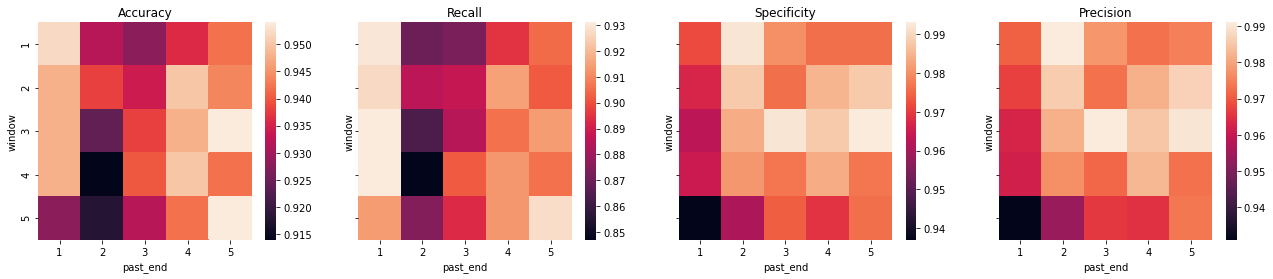
\includegraphics[width=1.3\textwidth]{res/res-fe-metrics}
            \caption{Die vier Metriken der Konfusionsmatrix.\vspace{1em}}
            \label{fig:res-fe-metrics}
        \end{subfigure}
        \begin{subfigure}{\textwidth}
            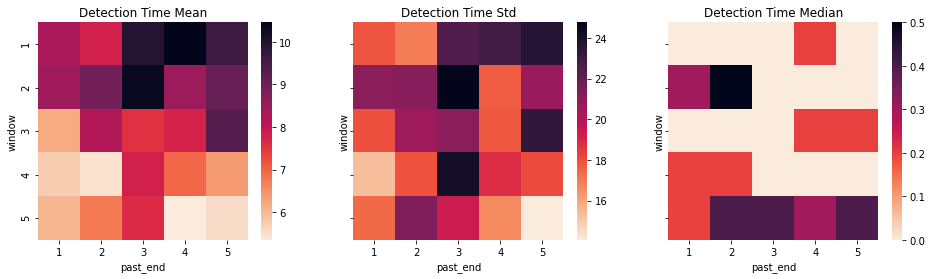
\includegraphics[width=0.9\textwidth]{res/res-fe-dt}
            \caption{Die Detektionszeit.}
            \label{fig:res-fe-dt}
        \end{subfigure}
        \caption{2-dimensionaler Verlauf durchschnittlicher Metrikwerte anhand der FE-spezifischen
            Hyperparameter \texttt{window} und \texttt{past\_end}. Hellere Werte sind hier besser.}
    \end{adjustwidth}
\end{figure}

\section{Diskussion \label{Chapter-Discussion}}

Um die Leistung verschiedener Ansätze des maschinellen Lernens in der Problemstellung der Leck-Detektion zu
 testen wurden diese zuerst auf einem einfachen und danach auf einem realistischeren Datensatz evaluiert. Dabei
 hat die Auswertung unter Anderem gezeigt, dass k-Nearest Neighbors sowohl im Ansatz der Klassifikation als auch
 des Regressions-Ensemble auf dem Ad-Hoc Datensatz beinahe perfekte Ergebnisse liefern kann, während es auf dem
 komplexen Datensatz stark schwächelt. Dies kann daran liegen, dass LeakDB neben den täglichen Schwankungen
 auch jährliche Veränderung besitzt, über die kNN keine Kenntnis haben kann. Die zusätzliche Angabe zum Beispiel
 der Kalenderwoche würde hier zwar vermutlich helfen, jedoch würde das viel mehr Daten erfordern. Zudem gibt es
 auch über Jahre hinweg andauernde Schwankungen durch das Weltklima, welche den Rahmen wieder sprengen würden.
 Die gegengesetzte Richtung, also dass Modelle auf den komplexeren Daten besser werden, ist bei den
 Regressionsalgorithmen zu sehen. Vor allem L2 kann hier signifikant an Sensitivität gewinnen. Ein möglicher
 Grund für die schlechtere Leistung auf den einfacheren Daten ist, dass diese anfangen, das Rauschen zu lernen,
 Stichwort Overfitting.

Ein weiterer großer Vorteil des Regression-Ensemble-Ansatzes ist, dass der Trainingsprozess nur leckfreie Daten
 benutzt. Das Modell kann also vollkommen auf leckbehaftete Zeitpunkte verzichtet, welche in manchen Städten rar
 sind.

Wichtig anzumerken ist jedoch, dass in der momentanen Implementation des Ensembles der Trainingsschritt noch
 ausgebessert werden kann. So werden aktuell auf allen (leckfreien) Datenpunkten trainiert und direkt
 prognostiziert, um die Differenzen, welche dann die Thresholds ergeben, zu berechnen. Das bedeutet, dass
 bereits gelernte Daten abgefragt werden, was, wie in Kapitel \ref{Chapter-ML} bereits gesagt, Probleme mit
 sich ziehen kann. Separates Training mit Cross Validation und extra Mengen alleine für die Berechnung der
 Differenzen kann zukünftig helfen, wobei ein solches Vorgehen wieder einen höheren Bedarf an Daten mit sich zieht.

Weitere Fragen, die sich aus der Analyse ergeben, sind die der einzelnen Hyperparameter. Betrachtet man
 \texttt{th\_majority}, so lässt sich das Absteigen von Sensitivität und Akkuratheit leicht erklären: Denn dieser
 Hyperparameter gibt die Anzahl an, wie viele Knoten Alarm schlagen müssen und erhöht damit die generelle Hürde,
 damit ein Zeitpunkt als Leck erklärt wird. Höhere Hürde trotz konstanter Werte führt zu geringeren Zahlen.
 Interessant ist jedoch die Präzision, welche zuerst stetig bei 100\% bleibt und dann plötzlich auf 0\%
 fällt. Aufschluss über dieses Verhalten gibt die Spezifität, welche hier bei 100\% liegt. Dieser Wert kann
 nur erreicht werden, wenn die Anzahl fälschlicherweise als positiv markierten Punkte (FP) gleich 0 ist.
 Für die Präzision, welche als $\frac{TP}{TP+FP}$ berechnet wird, bedeutet dies, dass sie nur die Werte 1, falls
 es mindestens ein richtigerweise positiv markierten Punkt gibt, oder 0, falls TP = 0 ist, erreichen
 kann\footnote{Bei TP = 0 würde die Formel zu $\frac{0}{0}$ evaluieren, was nicht definiert ist. Für diese Anwendung
 ist es jedoch als 0 definiert.}, was dieses Verhalten der Präzisionskurve erklärt. Die Werte zwischen 0 und 1
 stammen dabei aus der Mittelung der verschiedenen Konfigurationen. Bezüglich des Erhöhen der Hürde ist die
 Interaktion mit dem Hyperparameter \texttt{th\_multiplier} interessant. Da dessen Erhöhung ebenfalls eine
 Verstärkung der Hürde darstellt, könnte man meinen, dass diese Parameter in einer inversen Korrelation
 zueinander stehen sollten: So niedriger der Threshold, desto mehr Knoten sollte es zum Alarm schlagen
 benötigen. Doch die Abbildung \ref{fig:res-th-multiplier} unterstützt diese These nicht.

Betrachtet man die Aktivierungsfunktion des MLPs, so kann die gleiche Erklärung wie für den plötzlichen Abfall
 der Präzision bei \texttt{th\_majority} genutzt werden: Hier ist die Spezifität auch nahe 100\%, was für die
 logistische Funktion oder den Hyperbeltangens bedeutet, dass keine Zeitpunkte als Leck gelabelt wurden. Um
 den Einfluss der verborgenen Schichten eines MLPs genauer bestimmen zu können, muss dieser jedoch noch weiter
 getestet und analysiert werden. Für diese Tests wurde die Form zufällig gesampelt, das heißt, es wurden nicht
 alle Kombinationen ausgetestet. Vielleicht kann mit einer erschöpfenden Suche ein Besserer Zusammenhang
 gefunden werden.

Die Betrachtung der Detektionszeit zeigt keinen großen, von der der anderen Metriken abweichenden,
 Handlungsbedarf an. Der Unterschied in den gezeigten Beispielen betrifft meist nur unter zwei Zeitschritten,
 also bei LeakDB eine Stunde. Der maximale Median betrifft für die Evaluation des Feature Extraction nur einen
 halben Zeitschritt, was einer viertel Stunde entspricht.

Die größte Limitation betrifft jedoch das zugrunde liegende WDN. Denn mit nur neun Knotenpunkten ist das
 benutzte “Net1” ein sehr kleines Netzwerk, wodurch die Ergebnisse, selbst bei realistischer Simulation, ein
 verfälschtes Bild abgeben können. Weiterführend sollten die Modelle somit auf größeren Netzwerken getestet
 evaluiert werden.

Auch das Auffassen des Themas als Vorhersageproblem von Zeitfolgen kann in weiterer Forschung noch stärker
 exploriert werden, da die in dieser Arbeit betrachteten Algorithmen nur begrenzt zeitlichen Kontext inferieren
 können.

